\documentclass{article}
\usepackage{pythonhighlight}
\usepackage{graphicx}

% TITLE PAGE CONTENT %%%%%%%%%%%%%%%%%%%%%%%%
%%%%%%%%%%%%%%%%%%%%%%%%%%%%%%%%%%%%%%%%%%%%%
\newcommand{\labno}{01}
\newcommand{\labtitle}{EE208 Parser}
\newcommand{\authorname}{Zhou Litao}
\newcommand{\studentno}{518030910407}
\newcommand{\classno}{F1803016}
% END TITLE PAGE CONTENT %%%%%%%%%%%%%%%%%%%%


\begin{document}

\begin{center}
{\LARGE \textsc{Laboratory No. \labno:} \\ \vspace{4pt}}
{\Large \textsc{\labtitle} \\ \vspace{4pt}} 
\rule[13pt]{\textwidth}{1pt} \\ \vspace{15pt}
{\large By: \authorname \\ \vspace{10pt}
No. \studentno \\ \vspace{10pt}
SJTU \classno \\ \vspace{10pt}
\today \vspace{20pt}}
\end{center}



\section{Introduction}

\subsection{Equipment}
\begin{itemize}
\item\textbf{Environment} Ubuntu 16.04 (on Virtual Machine)
\item\textbf{Language} Python 2.7.16 with packages as follows
	\begin{itemize}
	\item urllib 1.24.2
	\item beautifulsoup4 4.8.0
	\end{itemize}
\item\textbf{Tools} PyCharm 2019.2, Virtual Box
\end{itemize}
The Python script is also tested in Windows 10.

\subsection{Purpose}
In this experiment, we're going to build a web-page parser. Three functions need to be implemented. First, the parser should be able to extract all the URLs from an arbitrary-given page and return a set of the URLs. Second, the parser needs to be able to extract all the images from an arbitray-given page and return a set of all the pages' addresses. Finally, for the `Zhihu Daily' website, the parser can output the image address, description text, and the linked page address for every piece of news. The experiment is based on some well-defined modules (such as \textit{BeautifulSoup, urllib}, etc.) in Python. The Python script should also be able to be executed in console.




\subsection{Principle}
HTML Parsers are used to extract contents from a given web-page according to its HTML labels, and organize them into a particular data structure. In this experiment, this work has already been done by the BeautifulSoup module. It takes in a webpage and return an HTML tree, which will be easier and more efficient for us to search for what we want.

As the flowchart depicts, our program should first get the HTML document according to the input URL, then we leave the parsing work for BeautifulSoup. With the HTML tree returned, we can use the built-in function to retrieve our objective information. Finally, some data processing work is needed before the program returns the values. Note that both the retrieval conditions and the data processing codes will vary in every exercise and should be carefully designed in order to fit the requirements.

\begin{figure}[htbp]
\centering
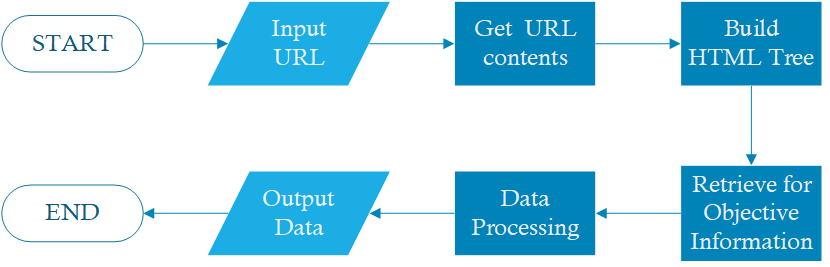
\includegraphics[width=9.5cm]{img/flowchart.png}
\label{fig:flowchart}
\caption{Flow Chart of the Lab}
\end{figure}

\section{Procedure}
\subsection{Exercise 1}

\subsubsection{Solution}
In this exercise, our goal is to return all the URLs (in the form of <a href...>) from a given page. With the HTML tree built by BeautifulSoup, all we have to do is to fetch all the URLs from the tree. First, we should locate to the <a> label and get the URL from its `href' property.

\paragraph{URL Matching} According to HTML standards, the `href' property can be a URL (with or without fragment identifiers), or a JavaScript segment. In order to distinguish URL from others, a Regular Expression is used here to match URLs. A remarkable characteristic in standard URL is that it begins with a protocol name which ends with `://'. So the Regular Expression can simply just check whether the property includes `://'   so as to exclude JavaScript segments out. Since the contents to be sorted is limited, this easy Regular Expression is considered to be enough for our sorting work.

\paragraph{Fragment Identifier Processing} Fragment identifiers are allowed in URL expressions, which can be introduced by a hash mark at the end of a URL. It is typically used to identify a portion of that document. For web crawlers, however, this part of the URL is unnecessary, since whether a URL has a fragment identifier or not, it indicates the same page. Therefore, for every URL we have collected, a string-processing step is designed to remove the identifier part. When the URL is added to the set, overlapping ones will be ignored. Another thing to note is that string.strip() is used to remove the whitespace at the head or end of the URL so that the URLs are uniformed.

\paragraph{About Protocol-relative URLs} Protocal-relative URLs begins with `//', indicating that the page it links uses the same protocal as the current page. They point to real pages that store information, and should be collected. However, due to the limitation of our function interface, there is no way to know the original URL of the current HTML document in the function body. Hence, non-standard URLs are aborted in this exercise.

The solutions above are implemented in the Python script as follows.
\begin{python}
def parseURL(content):
    urlset = set()
    soup = BeautifulSoup(content,features='html.parser')
    for i in soup.findAll('a',{'href': re.compile('://')}):
        j = i['href'].split('#')[0].strip()
        urlset.add(j)
\end{python}

\subsubsection{Results}
The test results can be found at graph \ref{img:1.1} and \ref{img:1.2}.

\begin{figure}[htbp]
\centering
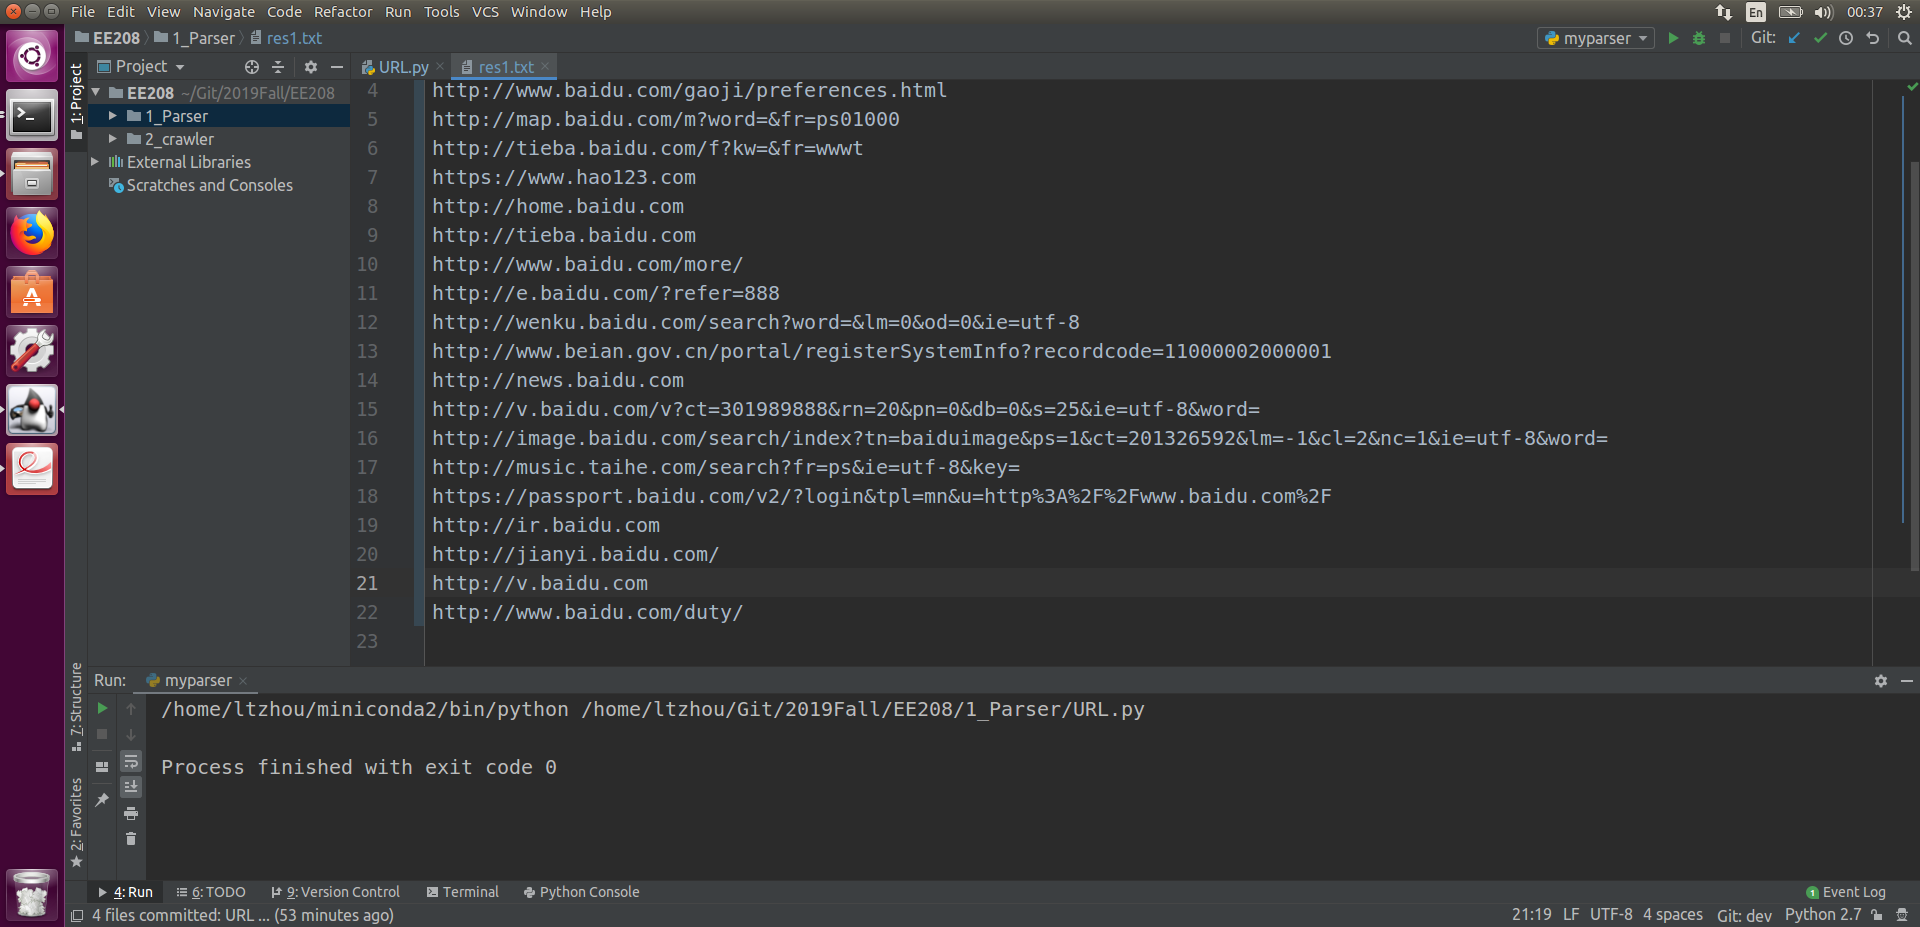
\includegraphics[width=9.5cm]{img/test1_1.png}
\caption{parseURL in PyCharm}
\label{img:1.1}
\end{figure}

\begin{figure}[htbp]
\centering
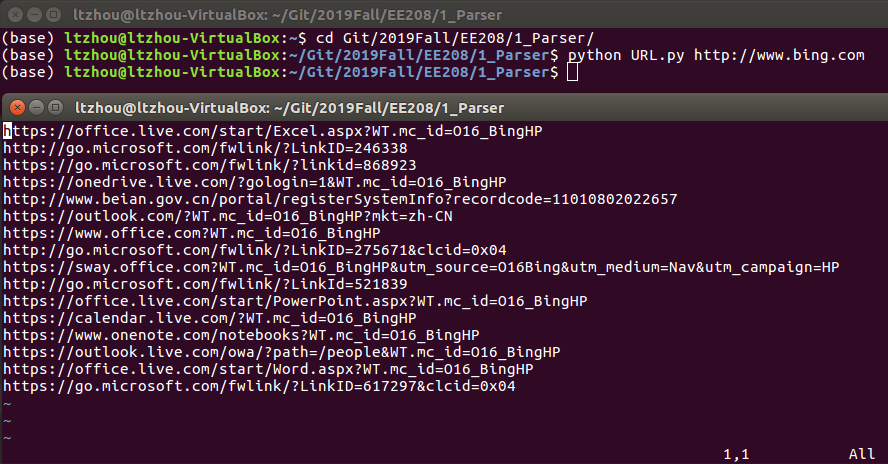
\includegraphics[width=9.5cm]{img/test1_2.png}
\caption{parseURL in console}
\label{img:1.2}
\end{figure}

\subsection{Exercise 2}

\subsubsection{Solution}

In this exercise, we should extract all the image addresses from the HTML tree. According to the requirement, we only need to consider the images in forms of <img src=``..">, so we first ask BeautifulSoup to fetch all the `src' properties in img labels. Also, for each address, we use string.split() for sake of uniformity. The codes of parseIMG are similar to parseURL, except that the findAll() condition is changed.

\begin{python}
    for i in soup.findAll('img'):
        imgset.add(i['src'].strip())
    return imgset
\end{python}

\paragraph{About Relative Paths} Similar to what we've discussed previously in Exercise 1, due to the lack of the original URL, it's hard to process relative paths within the parseIMG function. However, we can write a new function to process the relative paths. The codes of this function are listed as follows.

\begin{python}
def URL_set_uniform(URLset,url):
    urlseg = urlparse.urlparse(url)
    uniURLs = set()
    for j in URLset:
        if re.match('^//',j):         #case 1: relative-protocal URL
            uniURLs.add(urlseg.scheme+ ':'+j)
        elif (not re.match('://',j)): #case 2: relative path
            uniURLs.add(urlparse.urljoin(url,j))
        else:                         #case 3: standard URL
            uniURLs.add(j)
    return uniURLs
def main():
    ....
    urls = parseIMG(content)
    write_outputs(URL_set_uniform(urls,url), 'res2.txt')
\end{python}

Here, we import the urlparse module in Python in order to get the current URL scheme and deal with relative paths. First, urlparse() can split the URL into several meaningful parts, which includes the protocal of the current page. Then for every URL in the URLset, if the URL begins with `//' (i.e. relative-protocal URL), then we add the protocal before the string. If this is not the case and the URL can't match standard URL, then it should be a relative path. the urljoin() function can help us with the joining work. A new set is constructed in case of overlapping addresses after this operation. 

\subsubsection{Results}

The test results can be found at graph \ref{img:2.1} and \ref{img:2.2}.

\begin{figure}[htbp]
\centering
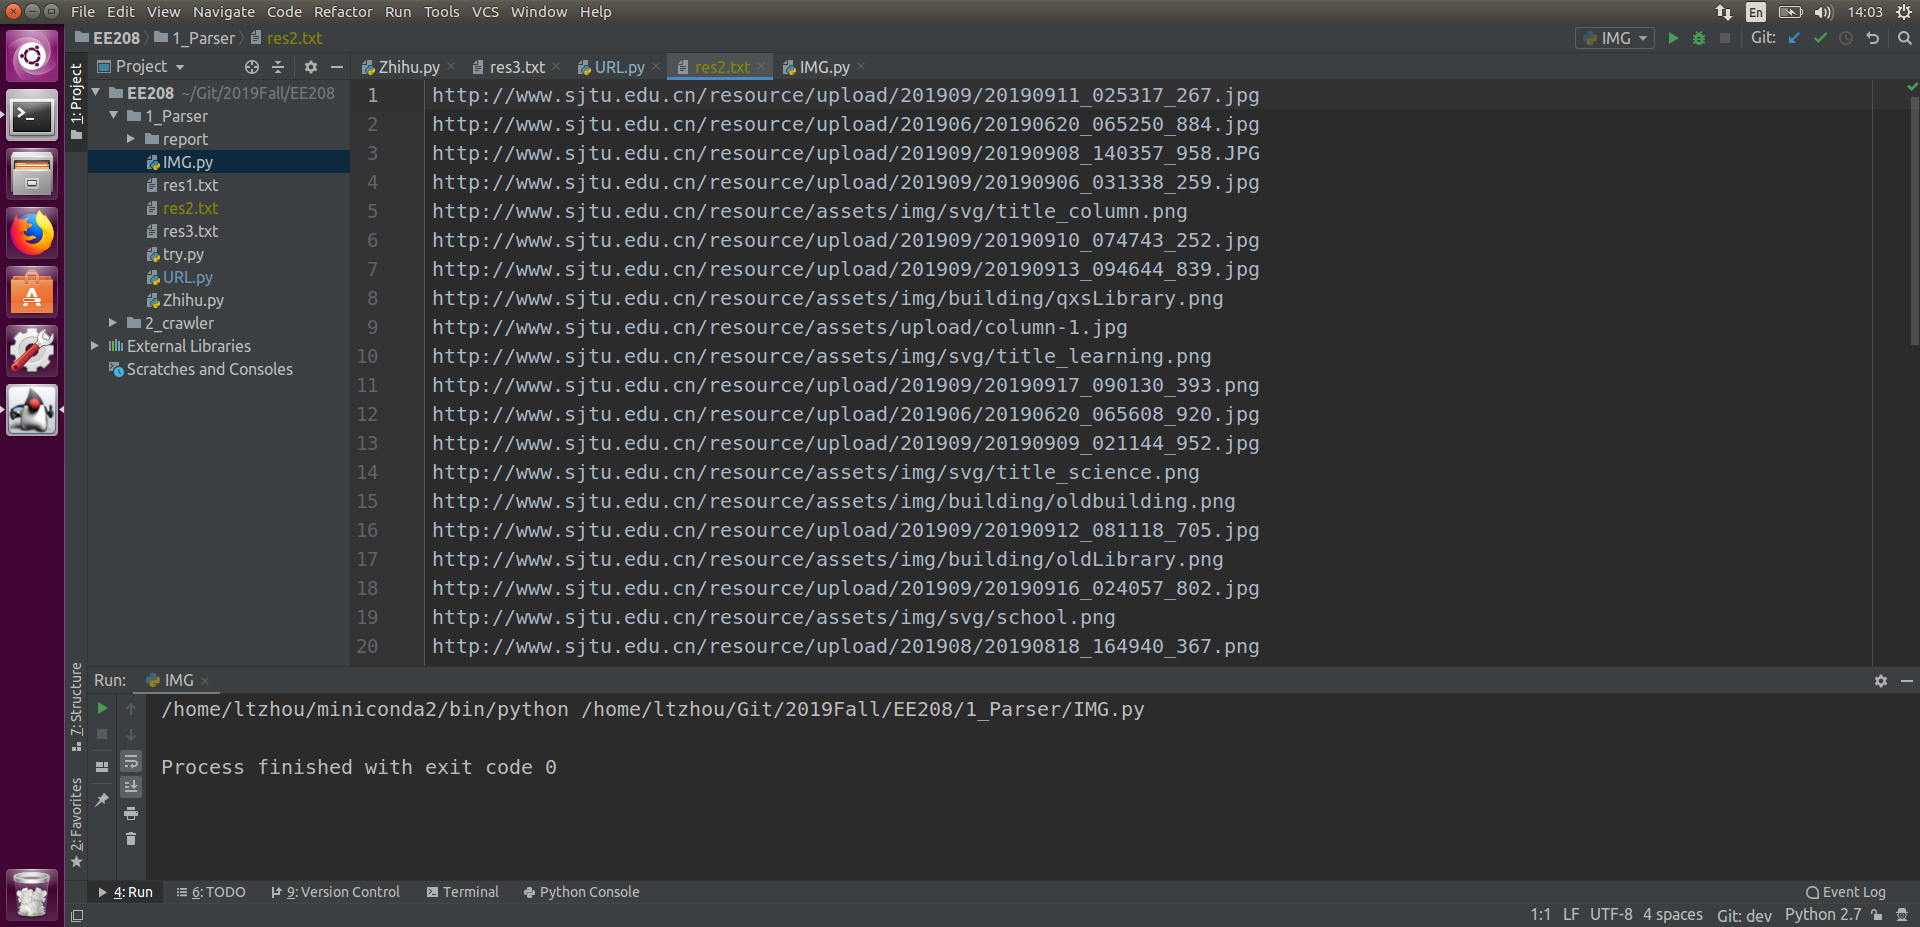
\includegraphics[width=9.5cm]{img/test2_1.png}
\caption{parseIMG in PyCharm}
\label{img:2.1}
\end{figure}

\begin{figure}[htbp]
\centering
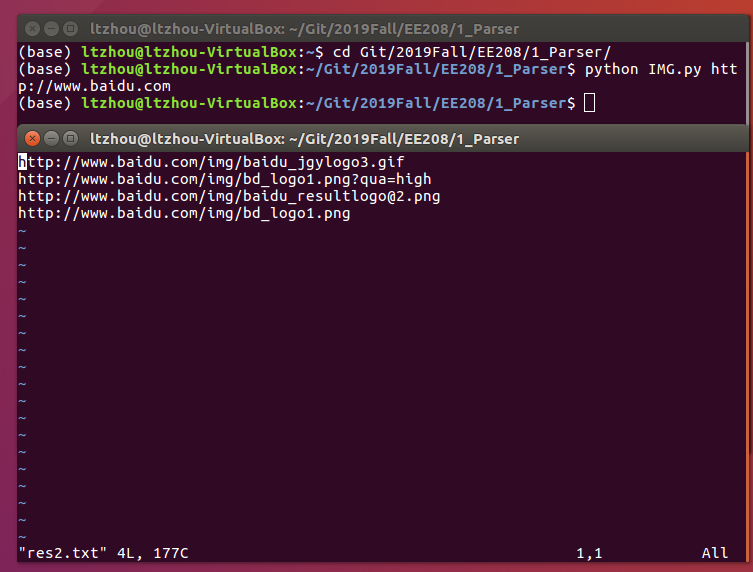
\includegraphics[width=9.5cm]{img/test2_2.png}
\caption{parseIMG in console}
\label{img:2.2}
\end{figure}



\subsection{Exercise 3}

\subsubsection{Solution}

By analyzing the information we want to extract, we can find that the contents to collect is located in a <div> named `box'. BeautifulSoup can easily locate to this <div> in the HTML tree. The findAll() command is written as follows

\begin{python}
def parseZhihuPic(url,content):
    pics = set()
    soup = BeautifulSoup(content,features='html.parser')
    divs = soup.findAll("div", "box")
    ...
\end{python}

Then by visiting the contents of this <div> node, we can collect the image addresses, text labels and URL link in every column. Note that the URL link here in Zhihu Daily is in the form of relative path. So when we are collecting the URL link, we change it into its full path. The 3 elements are packed in a tuple, and added into the result set.
\begin{python}
    for i in divs:
        pics.add((i.img['src'],i.span.string,url+i.a['href']))
    return pics
\end{python} 

In order to meet the requirement of the output format, we should rewrite the write\_outputs() function.
\begin{python}
def write_outputs(pics, filename):
    with open(filename, 'w') as f:
        for pic in pics:
            for j in range(3):
                f.write(pic[j])
                f.write('\n')
\end{python}

\subsubsection{Results}

In Exercise 3, no parameter in console is required. So whether in IDE or in console, the script will have the same effect. The test results can be found at graph \ref{img:3.1} and \ref{img:3.2}.

\begin{figure}[htbp]
\centering
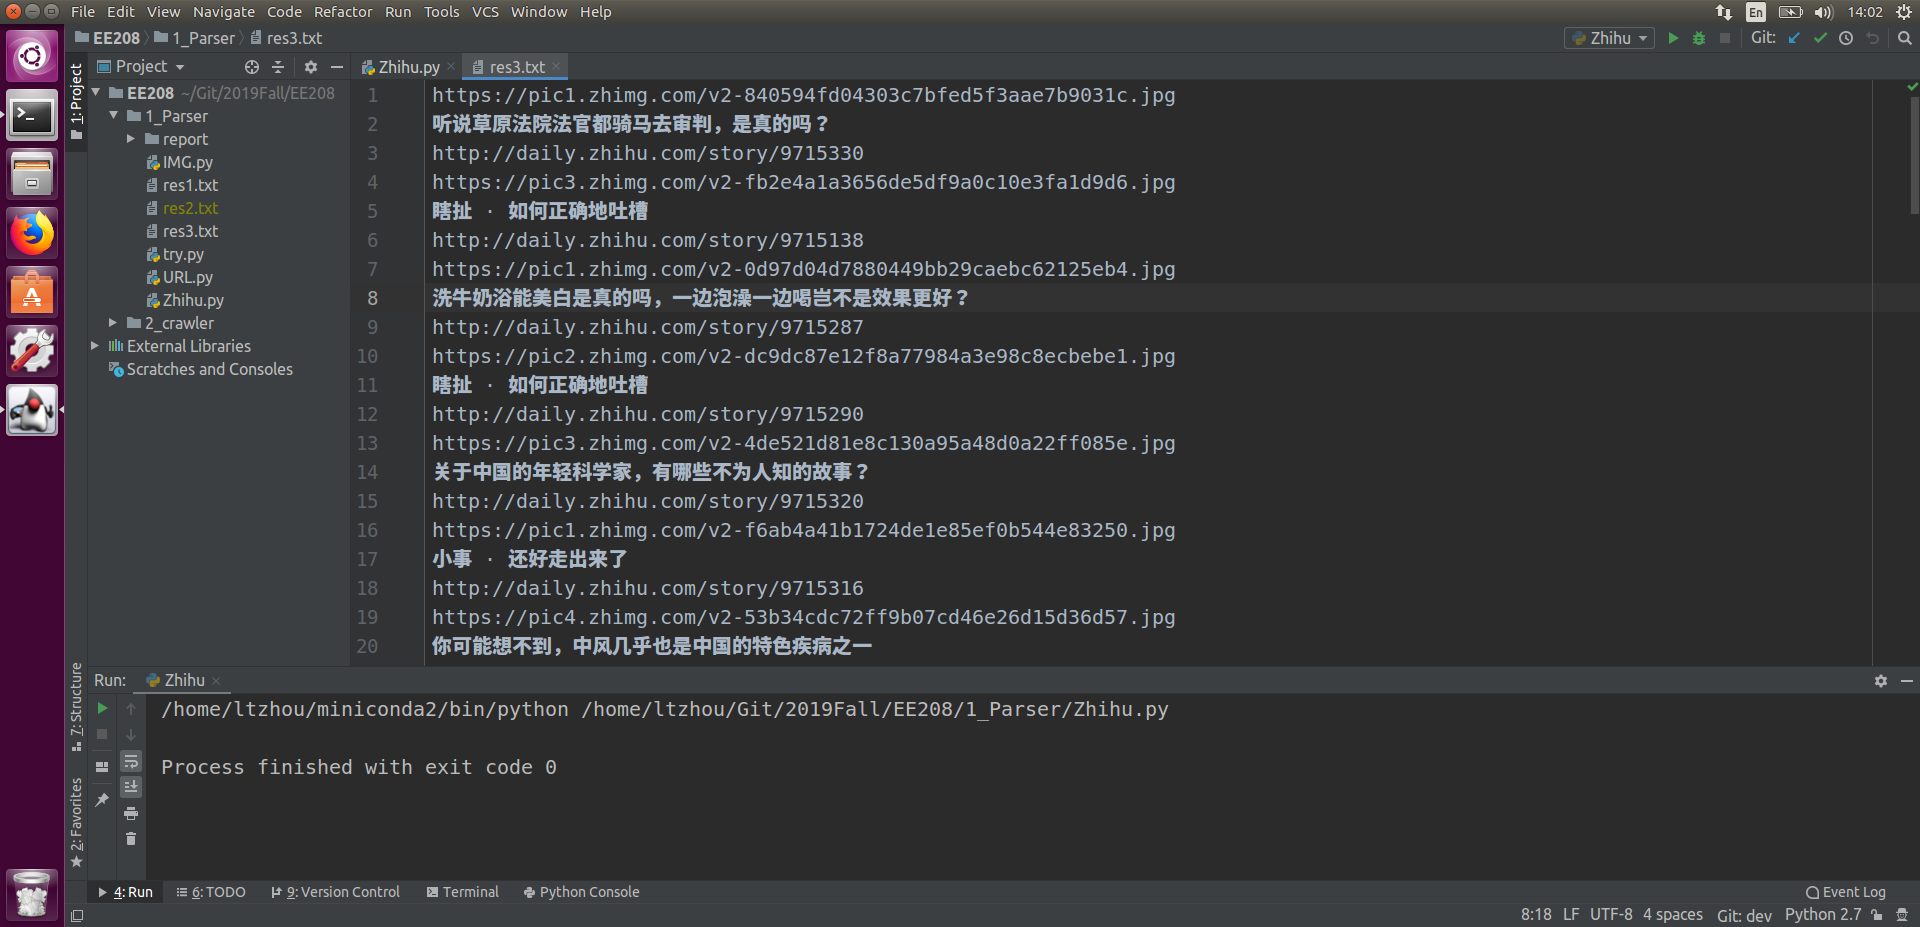
\includegraphics[width=9.5cm]{img/test3_1.png}
\caption{parseZhihuPic in PyCharm}
\label{img:3.1}
\end{figure}

\begin{figure}[htbp]
\centering
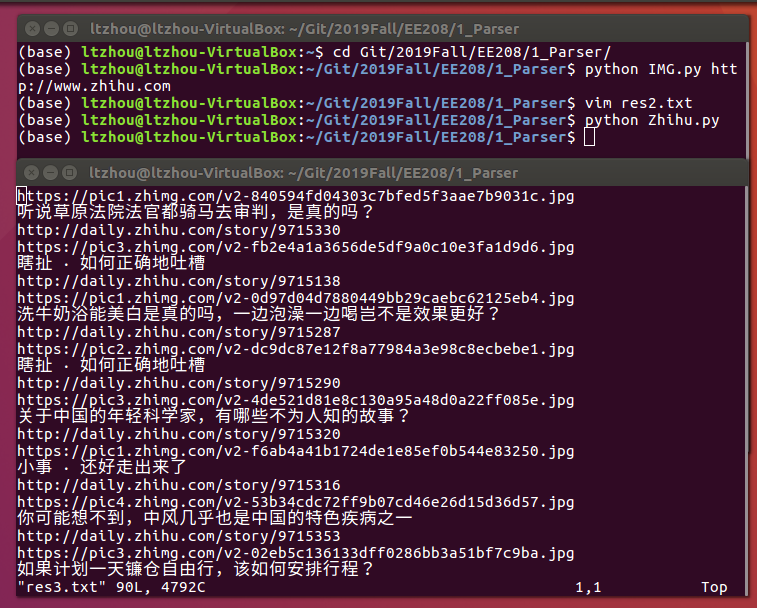
\includegraphics[width=9.5cm]{img/test3_2.png}
\caption{parseZhihuPic in console}
\label{img:3.2}
\end{figure}

\section{Discussion \& Conclusion}
\paragraph{Overview}
Through the practice of this laboratory, I have gained a general knowledge of how the HTML parser works and how we can make use of BeautifulSoup, a parser module in Python, to help us collect specific information from a webpage. I've also learnt some web data processing skills in the course of this lab.

\paragraph{Thoughts}
The structure and contents of different webpages vary a lot. When we are writing a parser project, it is important that we should bear in mind to "Make a concrete analysis of concrete conditions".  Only if we figure out how the contents are structured in the page can we locate our objective information correctly and efficiently. For example, in parseIMG, we should provide 3 cases based on how the image address looks like in order to return a satisfactory result.

\paragraph{Innovations}
In this lab, I have written a new useful function called URL\_ set\_uniform (See Exercise 2). Given a set of addresses (in the form of relative-protocal URLS, relative paths or standard URLs), it can return a set of addresses in their standard URL form. With this function, our functions can be more portable. I believe this will help a lot when we are dealing with further work such as crawlers.


\paragraph{Problems \& Solution}
The most encountered errors in this lab is about Coding. An efficient way to resolve this issue is to reload the sys module at the beginning of every Python script, as the following codes show.

\begin{python}
import sys
reload(sys)
sys.setdefaultencoding('utf-8')
\end{python}

\end{document}

